\appendix{Представление графического материала}

Графический материал, выполненный на отдельных листах,
изображен на рисунках А.1--А.\arabic{числоПлакатов}.
\setcounter{числоПлакатов}{0}

\renewcommand{\thefigure}{А.\arabic{figure}} % шаблон номера для плакатов

\begin{landscape}

\begin{плакат}
	
\includegraphics[width=0.82\linewidth]{list1.eps}
	\заголовок{Сведения о ВКРБ}
	\label{pl1:image}      
\end{плакат}

\begin{плакат}
	
\includegraphics[width=0.82\linewidth]{list2.eps}
	\заголовок{Цель и задачи}
	\label{pl2:image}      
\end{плакат}

\begin{плакат}
	
\includegraphics[width=0.82\linewidth]{list3.eps}
	\заголовок{Диаграмма прецедентов}
	\label{pl3:image}      
\end{плакат}

\begin{плакат}
	
\includegraphics[width=0.82\linewidth]{list4.eps}
	\заголовок{Оценка статистических параметров аугментированных данных}
	\label{pl4:image}      
\end{плакат}

\begin{плакат}
	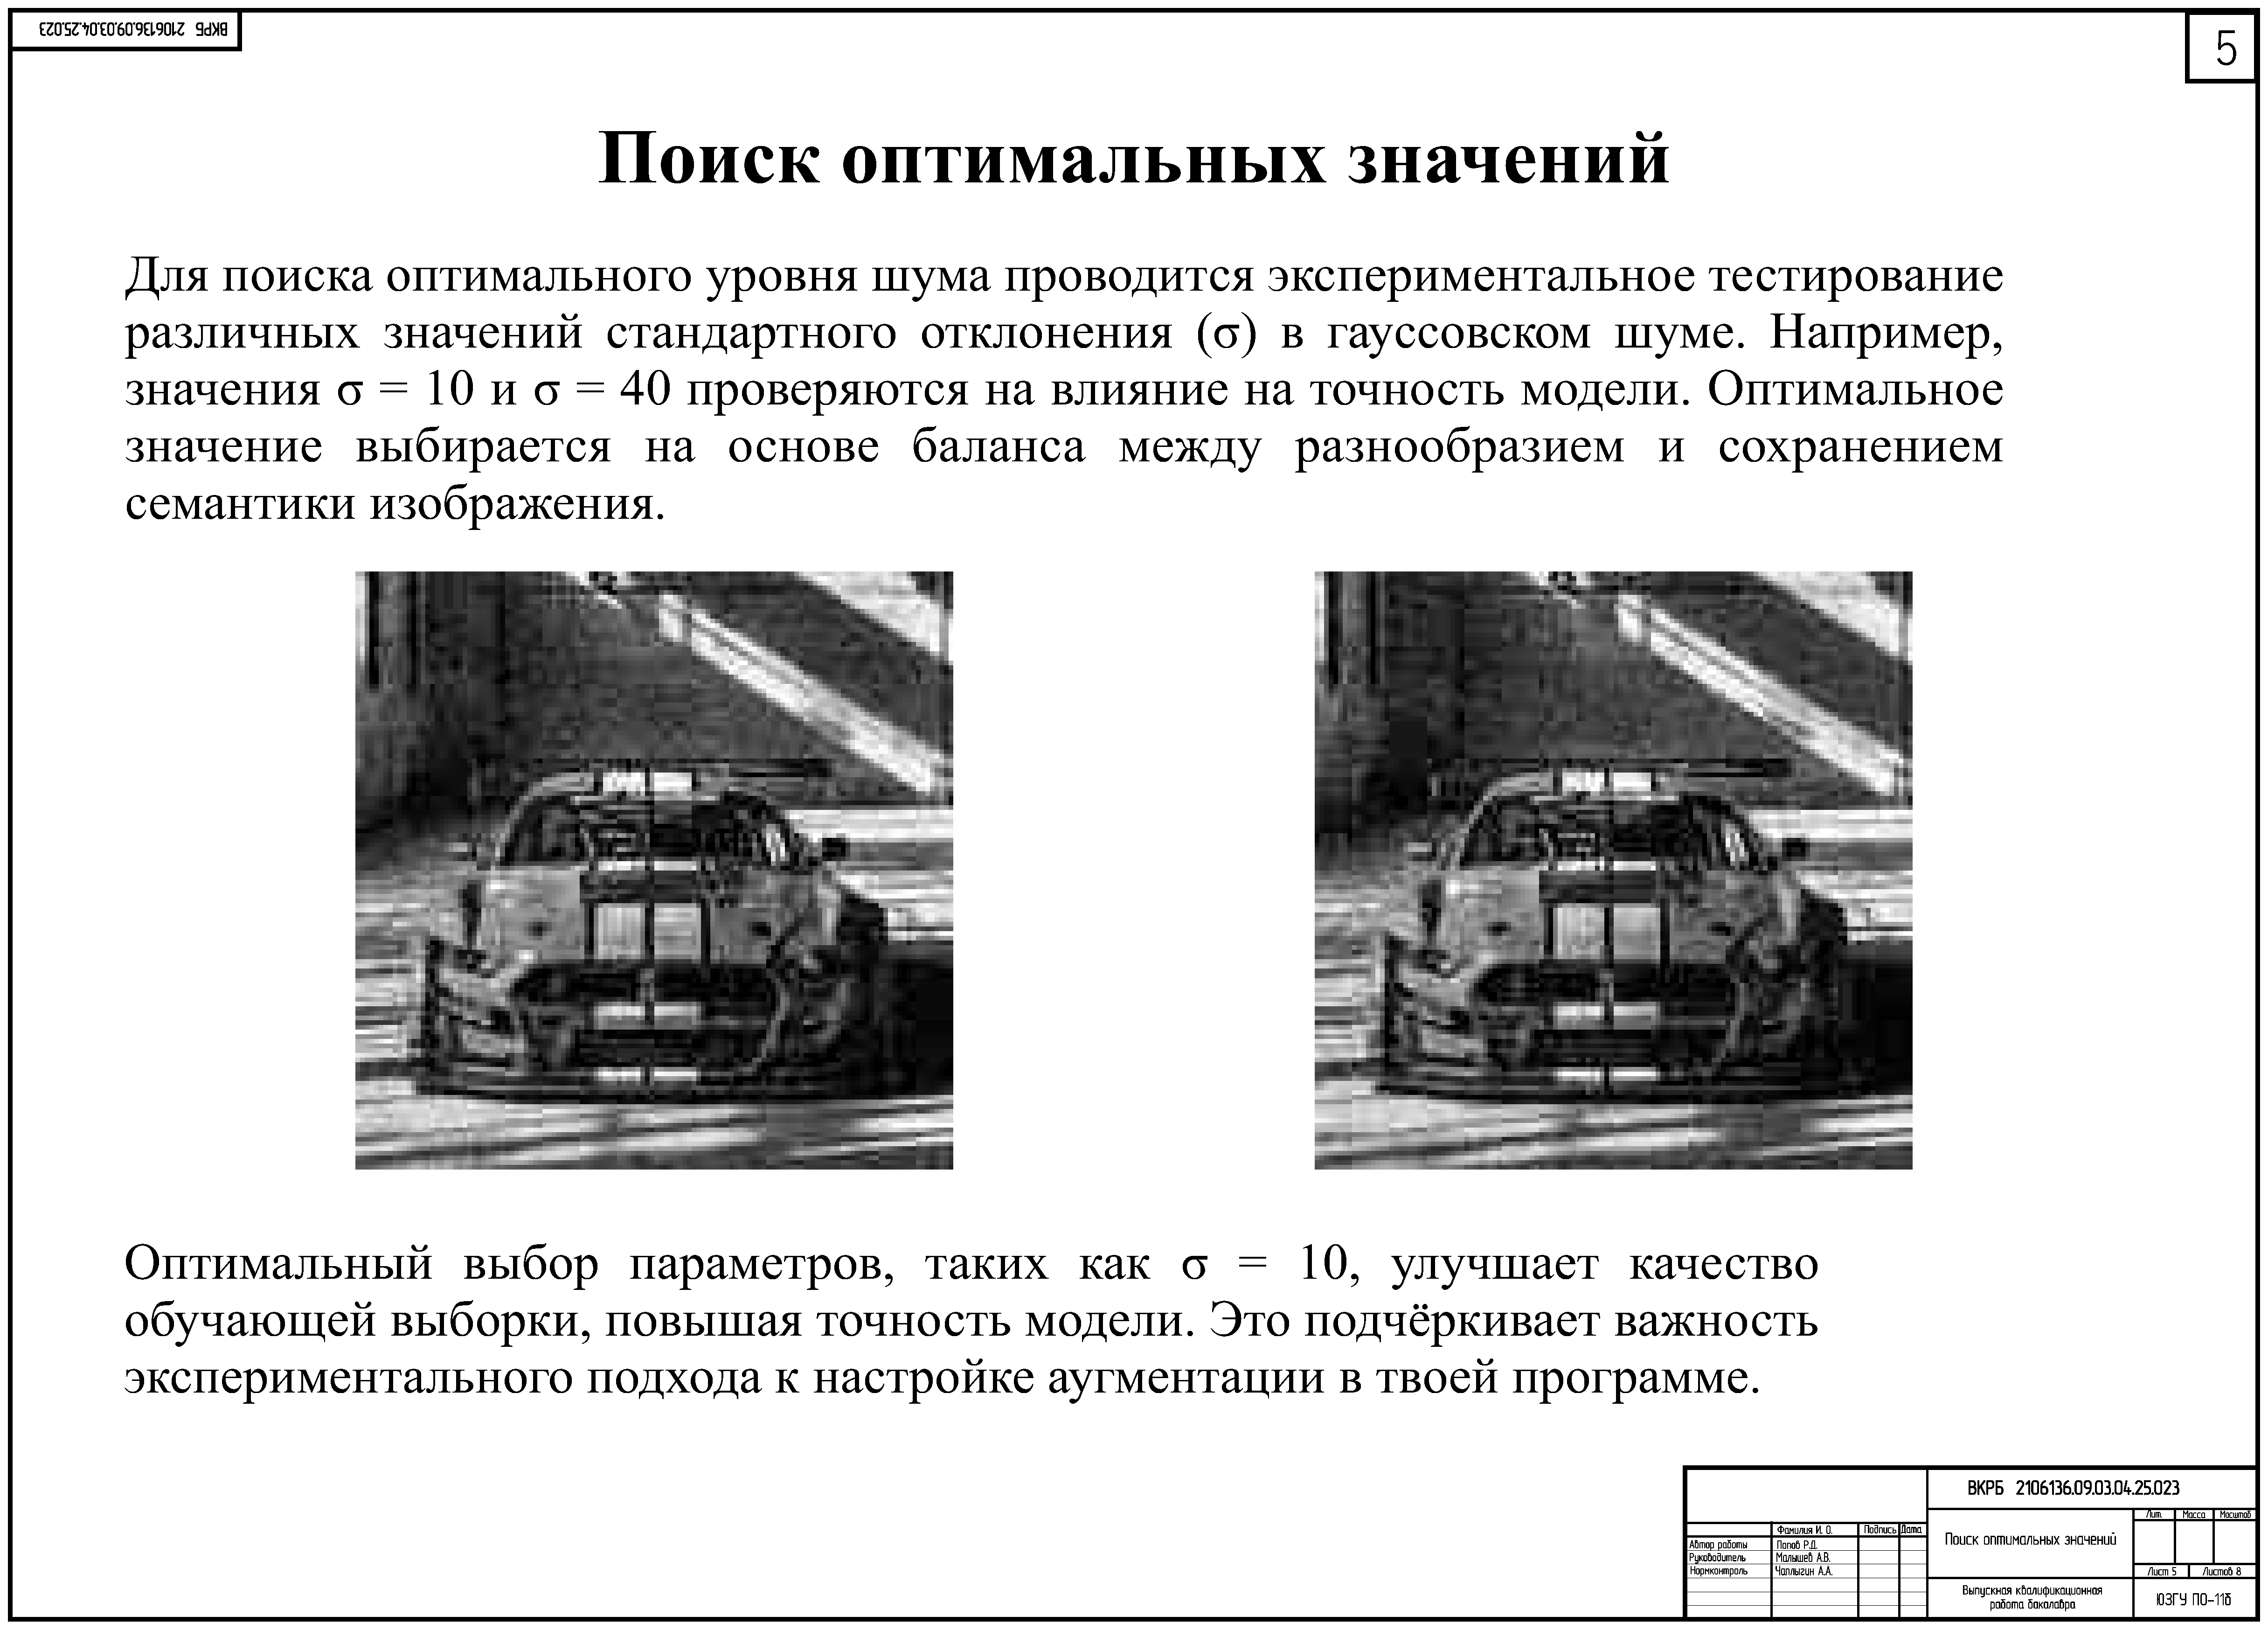
\includegraphics[width=0.82\linewidth]{list5.eps}
	\заголовок{Поиск оптимальных значений}
	\label{pl5:image}      
\end{плакат}

\begin{плакат}
	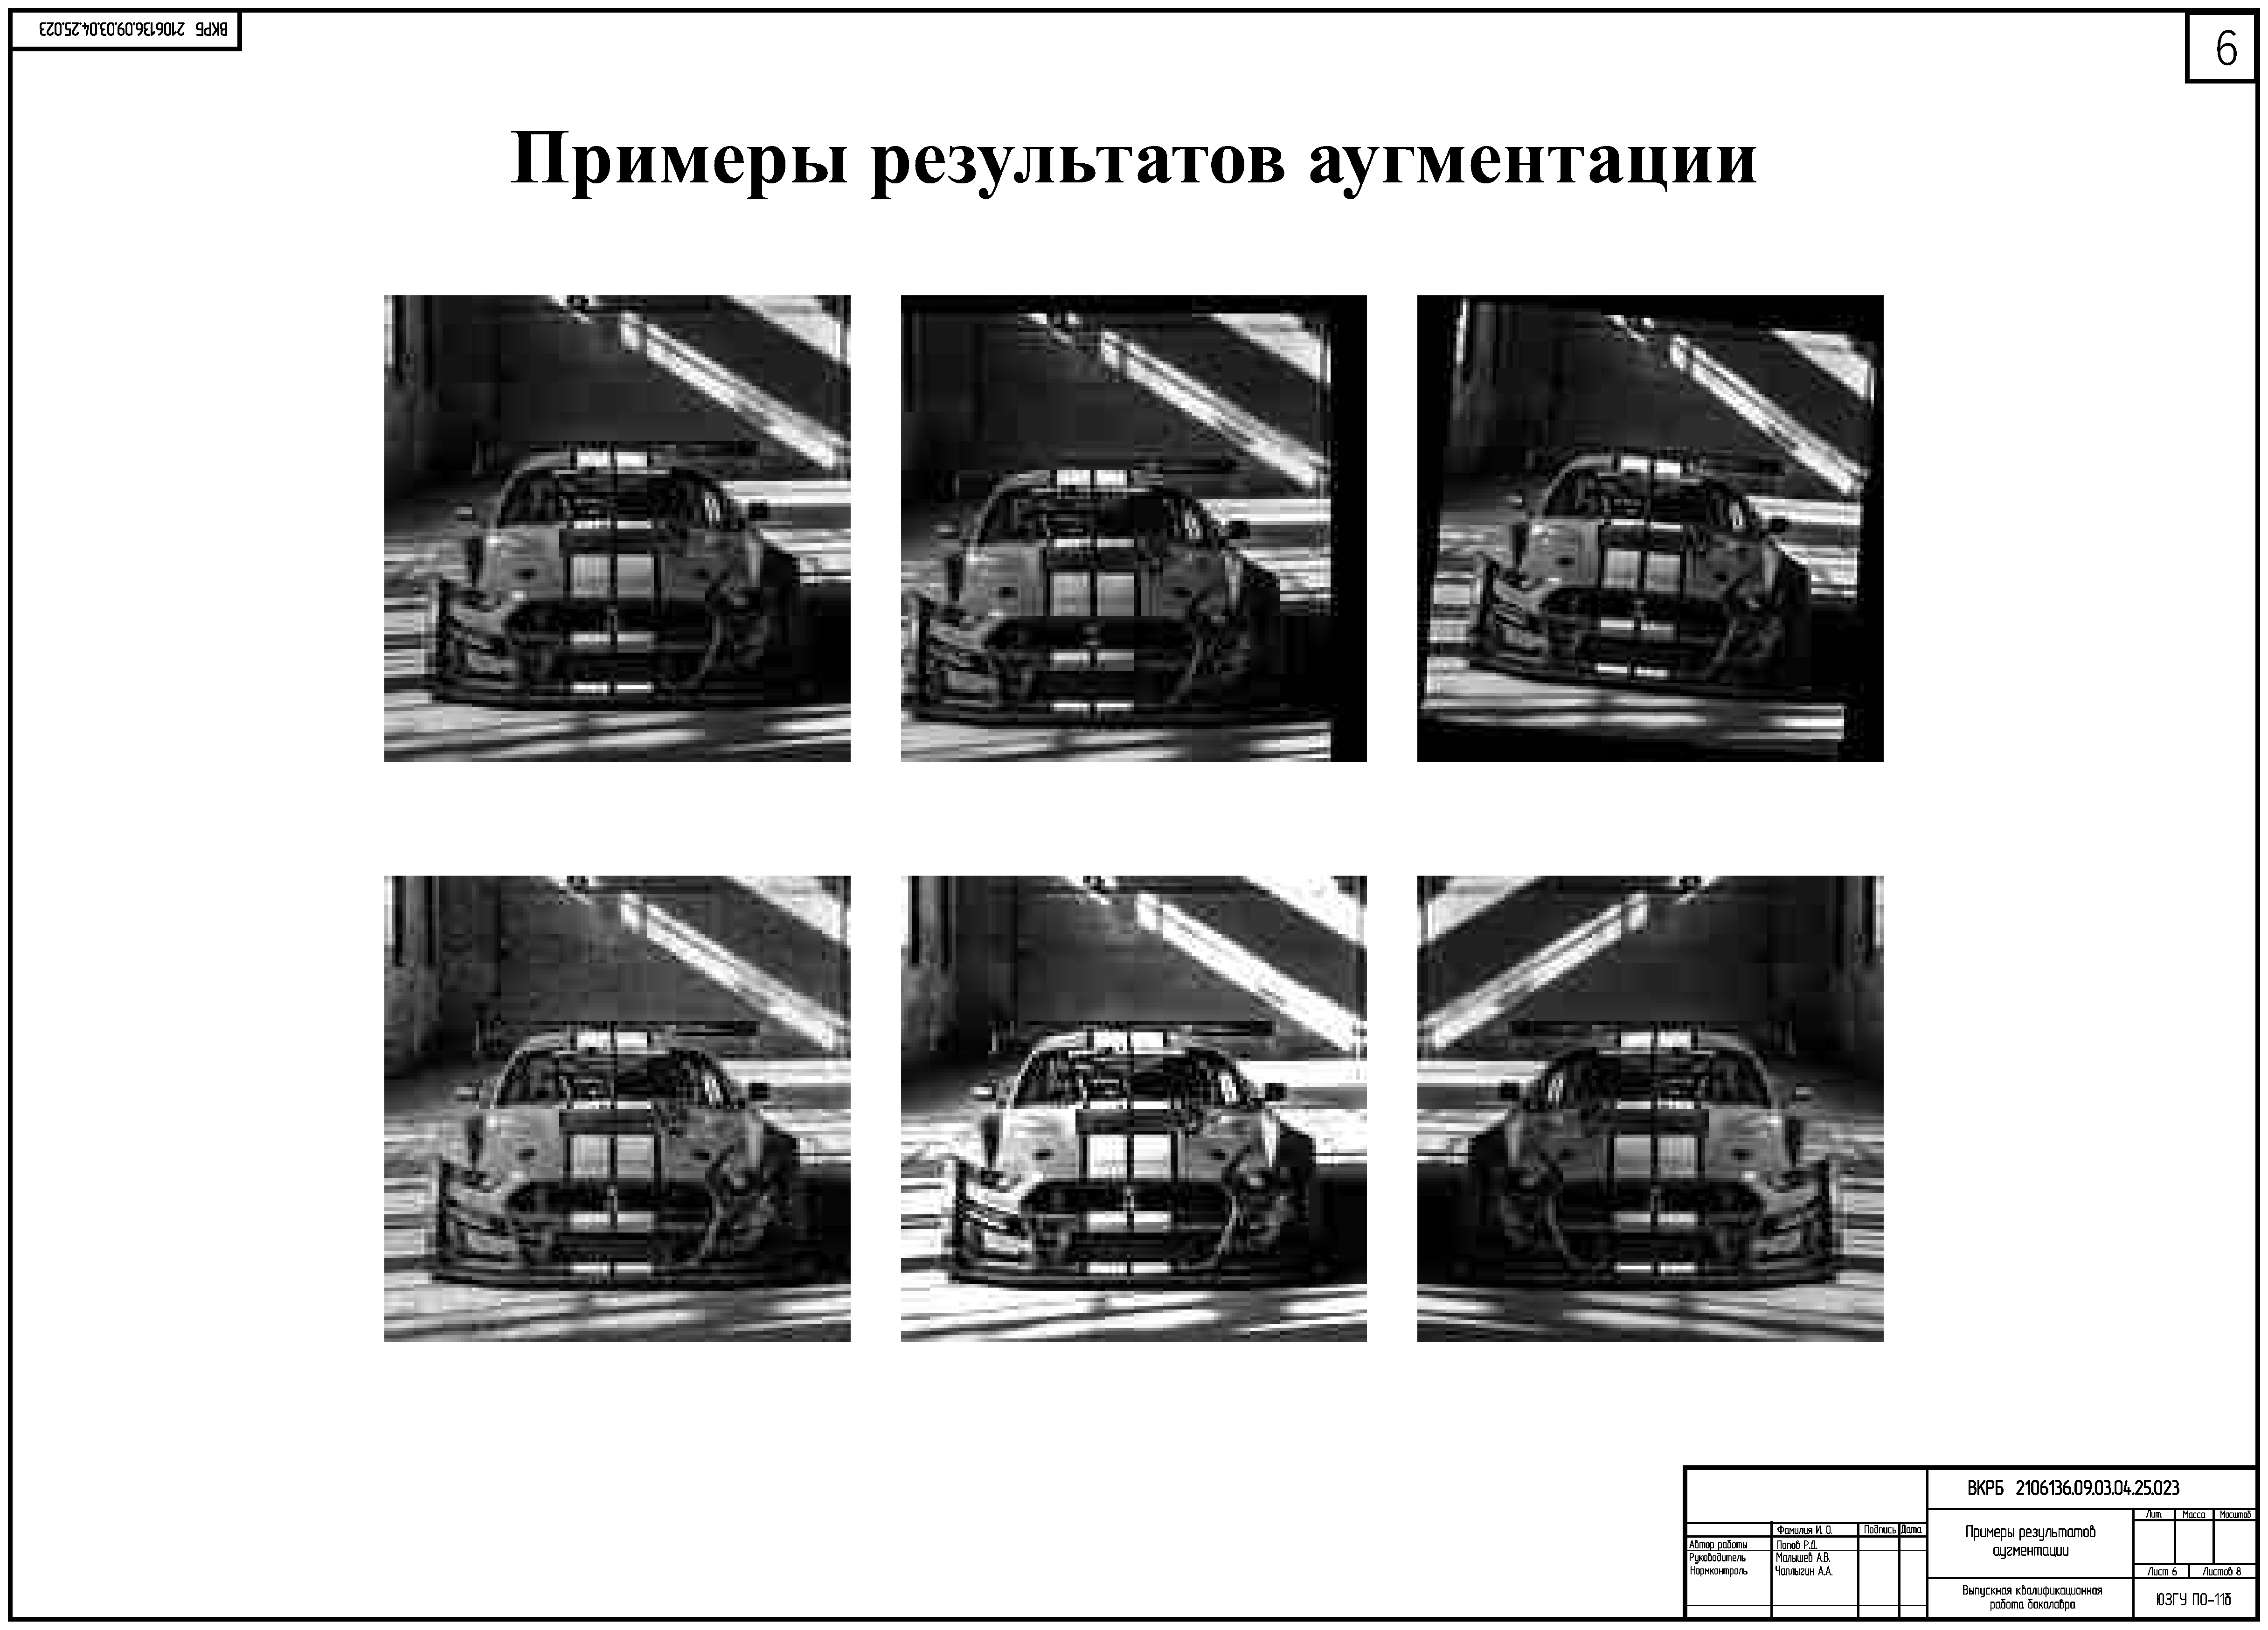
\includegraphics[width=0.82\linewidth]{list6.eps}
	\заголовок{Примеры результатов аугментации}
	\label{pl6:image}      
\end{плакат}

\begin{плакат}
	
\includegraphics[width=0.82\linewidth]{list7.eps}
	\заголовок{Интерфейс программы}
	\label{pl7:image}      
\end{плакат}

\begin{плакат}
	
\includegraphics[width=0.82\linewidth]{list8.eps}
	\заголовок{Заключение}
	\label{pl8:image}      
\end{плакат}


\end{landscape}
